
%----------------------------------------------------------------------------------------------------------------------------------------

% définit le type de document et ses options
\documentclass[a4paper,10pt]{article}

% des paquetages indispensables, qui ajoutent des fonctionnalites
\usepackage[utf8]{inputenc}
\usepackage{graphicx}
\usepackage{lscape}
\usepackage{url}
\usepackage{xspace}
\usepackage[francais]{babel}
%\usepackage{fullpage}

\pagestyle{plain}


%----------------------------------------------------------------------------------------------------------------------------------------


% le debut du contenu
\begin{document}


%----------------------------------------------------------------------------------------------------------------------------------------

%%%%%%%%%%%%%%%%%%%%%%%%%%%%%%%%%%%%%%%%%%%%%%%%%
%%Page d'accueil
\begin{center}
	%%
	\hspace{3cm}
	
\includegraphics[scale=0.8]{logo.ps}

	%%
	\vspace{1cm}
	{\large Projet de spécialité 2010}\\
	{\Large Conception d'un modèle de feu 3D temps réel}\\
	{\large Organisation du projet}\\
	\vspace{1cm}


	\includegraphics[scale=0.3]{feu.ps}\\
	\vspace{2cm}
	%%
	Etudiants impliqués :\\
	Benjamin Aupetit - IRVM - benjamin.aupetit@ensimag.imag.fr\\
	Julien Champeau - IRVM - julien.champeau@ensimag.imag.fr\\
	Arnaud Emilien - IRVM - arnaud.emilien@ensimag.imag.fr\\
	~\\
	Encadrants :\\
	Marie-Paule Cani  -  Marie-Paule.Cani@inrialpes.fr \\
	Aurélie Catel - aurelie.catel@grenoble-inp.fr
	~ \\
	\vspace{3mm}
	Ensimag 2010\\

\end{center}

\newpage

\tableofcontents

\newpage









%----------------------------------------------------------------------------------------------------------------------------------------
%%%%%%%%%%%%%%%%%
\section{Constitution de l'équipe}
%%%%%%%%%%%%%%%%%

\subsection{Choix du sujet}

Dans notre cursus IRVM nous avons assisté au cours "Graphique 3D" que nous avons particulièrement aprécié. Cette discipline est particulièrement indispensable à l'industrie du jeux vidéo, du film d'animation, ... \\
L'étude d'un phénomène réel, la conception de son modèle et la réalisation d'une application 3D temps réel est un procédé qui nous interesse particulièrement. Actuellement, aucun des sujets présentés ne propose cette démarche.\\
Cette discipline est d'autant plus importante pour nous que nous souhaitons en faire notre métier. Le projet de spécialité est une occasion unique de travailler à temps plein sur une problématique passionante, qui nous permettrait d'aquérir un savoir et des compétences importantes. Ce serait une réelle valeur ajouté dans notre bagage scolaire.\\
~\\
La modélisation du feu est un domaine interessant car il fait le lien entre de nombreux principes physiques, de nombreux modèles mathématiques, de nombreuses méthodes de calcul et de rendu. De plus la contrainte temps réel permet de ne garder que les éléments importants pour la visualisation, en simplifiant les modèles.


\subsection{Choix des membres}
\subsubsection{Arnaud}
\subsubsection{Benjamin}
\subsubsection{Julien}


\subsection{Forces et faiblesses de l'équipe}


%----------------------------------------------------------------------------------------------------------------------------------------
%%%%%%%%%%%%%%%%%
\section{Charte de travail}
La charte de travail a été établie dans le but de réaliser le plus de
points de notre sujet dans les délais impartis.  \\

Nous avons réparti le travail de façon homogène entre les membres de
l'équipe.  Nous nous sommes mis d'accord sur notre façon de travailler
: chacun d'entre nous utilise son propre ordinateur, nous utilisons un
gestionnaire de version ( «git» ) et nous nous sommes mis d'accord sur
une convention de codage et de commentaire. \\

Avant, et après, chaque rencontre avec notre tutrice. Avant pour
établir l'ordre du jour, discuter des point à discuter et/ou mettre en
avant. Et après pour en faire un bilan sur le déroulement de la
réunion et en déduire des éventuels changements d'orientation. \\

Pour les horaires de travail nouas avons choisis de travailler tous
les jours sauf le dimanche, de 9h à 17h et nous avons décidé de faire
un mini bilan sur ce que nous avons fait à la fin de chaque journée.\\

Les rôles ont été définis ainsi, en prenant en compte les points forts
de chacun :\\

\begin{itemize}

\item \textbf{Arnaud}
\begin{itemize}
\item bonne connaissance d'openGL.
\end{itemize}
\quad \\

\item \textbf{Benjamin}
\begin{itemize}
\item bon niveau en C++
\item familier avec l'analyse de problèmes et la modélisation en UML
\end{itemize}
\quad \\

\item \textbf{Julien}
\begin{itemize}
\item les maths
\end{itemize}
\quad \\

\end{itemize}
%%%%%%%%%%%%%%%%%




%----------------------------------------------------------------------------------------------------------------------------------------
%%%%%%%%%%%%%%%%%
\section{Planning prévisionnel}
%%%%%%%%%%%%%%%%%

	\includegraphics[scale=0.8]{../Planning/GANTT.ps}
	
	\includegraphics[scale=0.8]{../Planning/Planning.ps}


%----------------------------------------------------------------------------------------------------------------------------------------
%%%%%%%%%%%%%%%%%
\section{Répartition du travail}
%%%%%%%%%%%%%%%%%


%----------------------------------------------------------------------------------------------------------------------------------------
%%%%%%%%%%%%%%%%%
\section{Déroulement du projet}
%%%%%%%%%%%%%%%%%

%----------------------------------------------------------------------------------------------------------------------------------------
%%%%%%%%%%%%%%%%%
\section{Compte rendu des réunions}
%%%%%%%%%%%%%%%%%
%%%%%%%%%%%%%%%%%
\subsection{Suivis du  20 mai 2010}
%%%%%%%%%%%%%%%%%
\subsubsection{Présents}
\textbf{Tuteur} : Marie Paule Cani \\
\textbf{Élèves} : Benjamin, Julien, Arnaud \\
\subsubsection{Sujet abordé}
\textbf{Définition du but et de l'échelle du projet} :  \\
se concentrer sur la propagation et la destruction des objets.\\
\textbf{Pistes à regarder} : \\
Jos Stam a fait de nombreux travaux à ce sujet, il faut regarder sur son site web de toronto. Par exemple : burning cross. Il a travaillé sur la représentation et  les modèles de feu temps réel.\\
Mathieu Desbrun à fait "Voxels On fire" et "Meshes On Fire", deux travaux sur la propagation temps réel du feu sur un objet.\\
Représentation du feu par voxels.


\textbf{Conseil sur la démarche} : \\
Reflechir beaucoup au BUT,
identifier les phénomènes importants,
lire beaucoup,
faire des résumés régulièrement.

\subsubsection{Prochain rendez vous}
Lundi 31, à 10h à l'INRIA.\\
Nous devrons y présenter le modèle de feu et de fumée.

%%%%%%%%%%%%%%%%%
\subsection{Suivis du  31 mai 2010}
%%%%%%%%%%%%%%%%%
\subsubsection{Présents}
\textbf{Tuteur} : Marie Paule Cani\\
\textbf{Élèves} : Benjamin, Julien, Arnaud \\
\textbf{Et aussi : un chercheur de l'INRIA} : puis Cyril Crassin \\
\subsubsection{Sujet abordé}
\textbf{Présentation de l'avancement du projet} :  \\
\textbf{Explication de l'implémentation, discussion à propos des modifications/améliorations à apporter} :  \\
\textbf{Discussions à propos du travail futur} :  \\
\textbf{Résolution des problèmes liés à la version GPU} :  \\
    Dans le but de nous aider à comprendre les problèmes de notre version GPU, 
    notre tutrice nous à fait rencontrer Cyril Crassin, un chercheur de l'inria qui
    a beaucoup travaillé sur le GPU. 

\subsubsection{Prochain rendez vous}\\
Le prochain rendez-vous sera fixé dans la semaine par mail. Il s'agira sans doute de ventredi 4 Juin.



%----------------------------------------------------------------------------------------------------------------------------------------
%%%%%%%%%%%%%%%%%
\section{Conclusion}
%%%%%%%%%%%%%%%%%



%----------------------------------------------------------------------------------------------------------------------------------------
%%%%%%%%%%%%%%%%%
\section{Annexes}
%%%%%%%%%%%%%%%%%


%----------------------------------------------------------------------------------------------------------------------------------------
\end{document}
